\documentclass[twoside]{book}

% Packages required by doxygen
\usepackage{calc}
\usepackage{doxygen}
\usepackage{graphicx}
\usepackage[utf8]{inputenc}
\usepackage{makeidx}
\usepackage{multicol}
\usepackage{multirow}
\usepackage{textcomp}
\usepackage[table]{xcolor}

% Font selection
\usepackage[T1]{fontenc}
\usepackage{mathptmx}
\usepackage[scaled=.90]{helvet}
\usepackage{courier}
\usepackage{amssymb}
\usepackage{sectsty}
\renewcommand{\familydefault}{\sfdefault}
\allsectionsfont{%
  \fontseries{bc}\selectfont%
  \color{darkgray}%
}
\renewcommand{\DoxyLabelFont}{%
  \fontseries{bc}\selectfont%
  \color{darkgray}%
}

% Page & text layout
\usepackage{geometry}
\geometry{%
  a4paper,%
  top=2.5cm,%
  bottom=2.5cm,%
  left=2.5cm,%
  right=2.5cm%
}
\tolerance=750
\hfuzz=15pt
\hbadness=750
\setlength{\emergencystretch}{15pt}
\setlength{\parindent}{0cm}
\setlength{\parskip}{0.2cm}
\makeatletter
\renewcommand{\paragraph}{%
  \@startsection{paragraph}{4}{0ex}{-1.0ex}{1.0ex}{%
    \normalfont\normalsize\bfseries\SS@parafont%
  }%
}
\renewcommand{\subparagraph}{%
  \@startsection{subparagraph}{5}{0ex}{-1.0ex}{1.0ex}{%
    \normalfont\normalsize\bfseries\SS@subparafont%
  }%
}
\makeatother

% Headers & footers
\usepackage{fancyhdr}
\pagestyle{fancyplain}
\fancyhead[LE]{\fancyplain{}{\bfseries\thepage}}
\fancyhead[CE]{\fancyplain{}{}}
\fancyhead[RE]{\fancyplain{}{\bfseries\leftmark}}
\fancyhead[LO]{\fancyplain{}{\bfseries\rightmark}}
\fancyhead[CO]{\fancyplain{}{}}
\fancyhead[RO]{\fancyplain{}{\bfseries\thepage}}
\fancyfoot[LE]{\fancyplain{}{}}
\fancyfoot[CE]{\fancyplain{}{}}
\fancyfoot[RE]{\fancyplain{}{\bfseries\scriptsize Generated on Tue Jul 21 2015 19\-:05\-:52 for raytracer by Doxygen }}
\fancyfoot[LO]{\fancyplain{}{\bfseries\scriptsize Generated on Tue Jul 21 2015 19\-:05\-:52 for raytracer by Doxygen }}
\fancyfoot[CO]{\fancyplain{}{}}
\fancyfoot[RO]{\fancyplain{}{}}
\renewcommand{\footrulewidth}{0.4pt}
\renewcommand{\chaptermark}[1]{%
  \markboth{#1}{}%
}
\renewcommand{\sectionmark}[1]{%
  \markright{\thesection\ #1}%
}

% Indices & bibliography
\usepackage{natbib}
\usepackage[titles]{tocloft}
\setcounter{tocdepth}{3}
\setcounter{secnumdepth}{5}
\makeindex

% Hyperlinks (required, but should be loaded last)
\usepackage{ifpdf}
\ifpdf
  \usepackage[pdftex,pagebackref=true]{hyperref}
\else
  \usepackage[ps2pdf,pagebackref=true]{hyperref}
\fi
\hypersetup{%
  colorlinks=true,%
  linkcolor=blue,%
  citecolor=blue,%
  unicode%
}

% Custom commands
\newcommand{\clearemptydoublepage}{%
  \newpage{\pagestyle{empty}\cleardoublepage}%
}


%===== C O N T E N T S =====

\begin{document}

% Titlepage & ToC
\hypersetup{pageanchor=false}
\pagenumbering{roman}
\begin{titlepage}
\vspace*{7cm}
\begin{center}%
{\Large raytracer }\\
\vspace*{1cm}
{\large Generated by Doxygen 1.8.5}\\
\vspace*{0.5cm}
{\small Tue Jul 21 2015 19:05:52}\\
\end{center}
\end{titlepage}
\clearemptydoublepage
\tableofcontents
\clearemptydoublepage
\pagenumbering{arabic}
\hypersetup{pageanchor=true}

%--- Begin generated contents ---
\chapter{Hierarchical Index}
\section{Class Hierarchy}
This inheritance list is sorted roughly, but not completely, alphabetically\-:\begin{DoxyCompactList}
\item \contentsline{section}{Geometric\-Object}{\pageref{class_geometric_object}}{}
\begin{DoxyCompactList}
\item \contentsline{section}{Plane}{\pageref{class_plane}}{}
\item \contentsline{section}{Sphere}{\pageref{class_sphere}}{}
\end{DoxyCompactList}
\item \contentsline{section}{Hit\-Rec}{\pageref{class_hit_rec}}{}
\item \contentsline{section}{Image\-Buffer\-P\-N\-G}{\pageref{class_image_buffer_p_n_g}}{}
\item \contentsline{section}{Pixel}{\pageref{struct_pixel}}{}
\item \contentsline{section}{Ray}{\pageref{class_ray}}{}
\item \contentsline{section}{Ray\-Tracer}{\pageref{class_ray_tracer}}{}
\begin{DoxyCompactList}
\item \contentsline{section}{Multi\-Objects}{\pageref{class_multi_objects}}{}
\item \contentsline{section}{Single\-Sphere}{\pageref{class_single_sphere}}{}
\end{DoxyCompactList}
\item \contentsline{section}{R\-G\-B\-Color}{\pageref{class_r_g_b_color}}{}
\item \contentsline{section}{View\-Plane}{\pageref{class_view_plane}}{}
\item \contentsline{section}{World}{\pageref{class_world}}{}
\end{DoxyCompactList}

\chapter{Class Index}
\section{Class List}
Here are the classes, structs, unions and interfaces with brief descriptions\-:\begin{DoxyCompactList}
\item\contentsline{section}{\hyperlink{class_geometric_object}{Geometric\-Object} }{\pageref{class_geometric_object}}{}
\item\contentsline{section}{\hyperlink{class_hit_rec}{Hit\-Rec} }{\pageref{class_hit_rec}}{}
\item\contentsline{section}{\hyperlink{class_image_buffer_p_n_g}{Image\-Buffer\-P\-N\-G} }{\pageref{class_image_buffer_p_n_g}}{}
\item\contentsline{section}{\hyperlink{class_multi_objects}{Multi\-Objects} }{\pageref{class_multi_objects}}{}
\item\contentsline{section}{\hyperlink{struct_pixel}{Pixel} }{\pageref{struct_pixel}}{}
\item\contentsline{section}{\hyperlink{class_plane}{Plane} }{\pageref{class_plane}}{}
\item\contentsline{section}{\hyperlink{class_ray}{Ray} }{\pageref{class_ray}}{}
\item\contentsline{section}{\hyperlink{class_ray_tracer}{Ray\-Tracer} }{\pageref{class_ray_tracer}}{}
\item\contentsline{section}{\hyperlink{class_r_g_b_color}{R\-G\-B\-Color} }{\pageref{class_r_g_b_color}}{}
\item\contentsline{section}{\hyperlink{class_single_sphere}{Single\-Sphere} }{\pageref{class_single_sphere}}{}
\item\contentsline{section}{\hyperlink{class_sphere}{Sphere} }{\pageref{class_sphere}}{}
\item\contentsline{section}{\hyperlink{class_view_plane}{View\-Plane} }{\pageref{class_view_plane}}{}
\item\contentsline{section}{\hyperlink{class_world}{World} }{\pageref{class_world}}{}
\end{DoxyCompactList}

\chapter{File Index}
\section{File List}
Here is a list of all files with brief descriptions\-:\begin{DoxyCompactList}
\item\contentsline{section}{raytracer/include/\hyperlink{_hit_rec_8h}{Hit\-Rec.\-h} }{\pageref{_hit_rec_8h}}{}
\item\contentsline{section}{raytracer/include/\hyperlink{_image_buffer_p_n_g_8h}{Image\-Buffer\-P\-N\-G.\-h} }{\pageref{_image_buffer_p_n_g_8h}}{}
\item\contentsline{section}{raytracer/include/\hyperlink{_ray_8h}{Ray.\-h} }{\pageref{_ray_8h}}{}
\item\contentsline{section}{raytracer/include/\hyperlink{_r_g_b_color_8h}{R\-G\-B\-Color.\-h} }{\pageref{_r_g_b_color_8h}}{}
\item\contentsline{section}{raytracer/include/\hyperlink{_view_plane_8h}{View\-Plane.\-h} }{\pageref{_view_plane_8h}}{}
\item\contentsline{section}{raytracer/include/\hyperlink{_world_8h}{World.\-h} }{\pageref{_world_8h}}{}
\item\contentsline{section}{raytracer/include/geom/\hyperlink{_geometric_object_8h}{Geometric\-Object.\-h} }{\pageref{_geometric_object_8h}}{}
\item\contentsline{section}{raytracer/include/geom/\hyperlink{_plane_8h}{Plane.\-h} }{\pageref{_plane_8h}}{}
\item\contentsline{section}{raytracer/include/geom/\hyperlink{_sphere_8h}{Sphere.\-h} }{\pageref{_sphere_8h}}{}
\item\contentsline{section}{raytracer/include/tracer/\hyperlink{_multi_objects_8h}{Multi\-Objects.\-h} }{\pageref{_multi_objects_8h}}{}
\item\contentsline{section}{raytracer/include/tracer/\hyperlink{_ray_tracer_8h}{Ray\-Tracer.\-h} }{\pageref{_ray_tracer_8h}}{}
\item\contentsline{section}{raytracer/include/tracer/\hyperlink{_single_sphere_8h}{Single\-Sphere.\-h} }{\pageref{_single_sphere_8h}}{}
\item\contentsline{section}{raytracer/source/common/\hyperlink{_hit_rec_8cpp}{Hit\-Rec.\-cpp} }{\pageref{_hit_rec_8cpp}}{}
\item\contentsline{section}{raytracer/source/common/\hyperlink{_image_buffer_p_n_g_8cpp}{Image\-Buffer\-P\-N\-G.\-cpp} }{\pageref{_image_buffer_p_n_g_8cpp}}{}
\item\contentsline{section}{raytracer/source/common/\hyperlink{_main_8cpp}{Main.\-cpp} }{\pageref{_main_8cpp}}{}
\item\contentsline{section}{raytracer/source/common/\hyperlink{_ray_8cpp}{Ray.\-cpp} }{\pageref{_ray_8cpp}}{}
\item\contentsline{section}{raytracer/source/common/\hyperlink{_r_g_b_color_8cpp}{R\-G\-B\-Color.\-cpp} }{\pageref{_r_g_b_color_8cpp}}{}
\item\contentsline{section}{raytracer/source/common/\hyperlink{_view_plane_8cpp}{View\-Plane.\-cpp} }{\pageref{_view_plane_8cpp}}{}
\item\contentsline{section}{raytracer/source/common/\hyperlink{_world_8cpp}{World.\-cpp} }{\pageref{_world_8cpp}}{}
\item\contentsline{section}{raytracer/source/common/geom/\hyperlink{_geometric_object_8cpp}{Geometric\-Object.\-cpp} }{\pageref{_geometric_object_8cpp}}{}
\item\contentsline{section}{raytracer/source/common/geom/\hyperlink{_plane_8cpp}{Plane.\-cpp} }{\pageref{_plane_8cpp}}{}
\item\contentsline{section}{raytracer/source/common/geom/\hyperlink{_sphere_8cpp}{Sphere.\-cpp} }{\pageref{_sphere_8cpp}}{}
\item\contentsline{section}{raytracer/source/common/tracer/\hyperlink{_multi_objects_8cpp}{Multi\-Objects.\-cpp} }{\pageref{_multi_objects_8cpp}}{}
\item\contentsline{section}{raytracer/source/common/tracer/\hyperlink{_ray_tracer_8cpp}{Ray\-Tracer.\-cpp} }{\pageref{_ray_tracer_8cpp}}{}
\item\contentsline{section}{raytracer/source/common/tracer/\hyperlink{_single_sphere_8cpp}{Single\-Sphere.\-cpp} }{\pageref{_single_sphere_8cpp}}{}
\end{DoxyCompactList}

\chapter{Class Documentation}
\hypertarget{class_geometric_object}{\section{Geometric\-Object Class Reference}
\label{class_geometric_object}\index{Geometric\-Object@{Geometric\-Object}}
}


{\ttfamily \#include $<$Geometric\-Object.\-h$>$}

Inheritance diagram for Geometric\-Object\-:\begin{figure}[H]
\begin{center}
\leavevmode
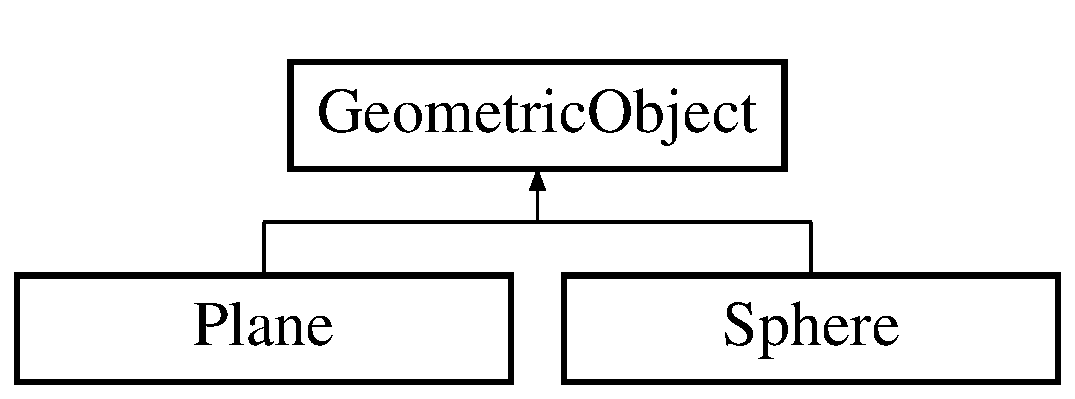
\includegraphics[height=2.000000cm]{class_geometric_object}
\end{center}
\end{figure}
\subsection*{Public Member Functions}
\begin{DoxyCompactItemize}
\item 
virtual bool \hyperlink{class_geometric_object_a6872aae2052bf80cdc0bd87191630b18}{Hit} (const \hyperlink{class_ray}{Ray} \&ray, double \&tmin, \hyperlink{class_hit_rec}{Hit\-Rec} \&hr) const =0
\item 
virtual \hyperlink{class_r_g_b_color}{R\-G\-B\-Color} \hyperlink{class_geometric_object_a5971a505ae42f3c916b1f5428b4b3ce1}{Get\-Base\-Color} ()=0
\end{DoxyCompactItemize}


\subsection{Member Function Documentation}
\hypertarget{class_geometric_object_a5971a505ae42f3c916b1f5428b4b3ce1}{\index{Geometric\-Object@{Geometric\-Object}!Get\-Base\-Color@{Get\-Base\-Color}}
\index{Get\-Base\-Color@{Get\-Base\-Color}!GeometricObject@{Geometric\-Object}}
\subsubsection[{Get\-Base\-Color}]{\setlength{\rightskip}{0pt plus 5cm}virtual {\bf R\-G\-B\-Color} Geometric\-Object\-::\-Get\-Base\-Color (
\begin{DoxyParamCaption}
{}
\end{DoxyParamCaption}
)\hspace{0.3cm}{\ttfamily [pure virtual]}}}\label{class_geometric_object_a5971a505ae42f3c916b1f5428b4b3ce1}


Implemented in \hyperlink{class_sphere_a1a1446f19a193f966cb04704faa3c3e8}{Sphere}.

\hypertarget{class_geometric_object_a6872aae2052bf80cdc0bd87191630b18}{\index{Geometric\-Object@{Geometric\-Object}!Hit@{Hit}}
\index{Hit@{Hit}!GeometricObject@{Geometric\-Object}}
\subsubsection[{Hit}]{\setlength{\rightskip}{0pt plus 5cm}virtual bool Geometric\-Object\-::\-Hit (
\begin{DoxyParamCaption}
\item[{const {\bf Ray} \&}]{ray, }
\item[{double \&}]{tmin, }
\item[{{\bf Hit\-Rec} \&}]{hr}
\end{DoxyParamCaption}
) const\hspace{0.3cm}{\ttfamily [pure virtual]}}}\label{class_geometric_object_a6872aae2052bf80cdc0bd87191630b18}


Implemented in \hyperlink{class_sphere_abfe41f348343d7d1dd4a6e5c384c615d}{Sphere}, and \hyperlink{class_plane_a51cf933b7cc15b48fa155705d060c541}{Plane}.



The documentation for this class was generated from the following file\-:\begin{DoxyCompactItemize}
\item 
raytracer/include/geom/\hyperlink{_geometric_object_8h}{Geometric\-Object.\-h}\end{DoxyCompactItemize}

\hypertarget{class_hit_rec}{\section{Hit\-Rec Class Reference}
\label{class_hit_rec}\index{Hit\-Rec@{Hit\-Rec}}
}


{\ttfamily \#include $<$Hit\-Rec.\-h$>$}

\subsection*{Public Member Functions}
\begin{DoxyCompactItemize}
\item 
\hyperlink{class_hit_rec_a1f1da80530a358dc8592d5d8cd0401e0}{Hit\-Rec} ()
\end{DoxyCompactItemize}
\subsection*{Public Attributes}
\begin{DoxyCompactItemize}
\item 
bool \hyperlink{class_hit_rec_a7b6523b2c80ecb6c74e842e6f0e141bc}{did\-Hit}
\item 
glm\-::vec3 \hyperlink{class_hit_rec_af469c5c83f30778acc72e52161304b0e}{hit\-Point}
\item 
glm\-::vec3 \hyperlink{class_hit_rec_ae3497f607cf5bc135efe6a95f2f1518c}{normal}
\end{DoxyCompactItemize}


\subsection{Constructor \& Destructor Documentation}
\hypertarget{class_hit_rec_a1f1da80530a358dc8592d5d8cd0401e0}{\index{Hit\-Rec@{Hit\-Rec}!Hit\-Rec@{Hit\-Rec}}
\index{Hit\-Rec@{Hit\-Rec}!HitRec@{Hit\-Rec}}
\subsubsection[{Hit\-Rec}]{\setlength{\rightskip}{0pt plus 5cm}Hit\-Rec\-::\-Hit\-Rec (
\begin{DoxyParamCaption}
{}
\end{DoxyParamCaption}
)}}\label{class_hit_rec_a1f1da80530a358dc8592d5d8cd0401e0}


\subsection{Member Data Documentation}
\hypertarget{class_hit_rec_a7b6523b2c80ecb6c74e842e6f0e141bc}{\index{Hit\-Rec@{Hit\-Rec}!did\-Hit@{did\-Hit}}
\index{did\-Hit@{did\-Hit}!HitRec@{Hit\-Rec}}
\subsubsection[{did\-Hit}]{\setlength{\rightskip}{0pt plus 5cm}bool Hit\-Rec\-::did\-Hit}}\label{class_hit_rec_a7b6523b2c80ecb6c74e842e6f0e141bc}
\hypertarget{class_hit_rec_af469c5c83f30778acc72e52161304b0e}{\index{Hit\-Rec@{Hit\-Rec}!hit\-Point@{hit\-Point}}
\index{hit\-Point@{hit\-Point}!HitRec@{Hit\-Rec}}
\subsubsection[{hit\-Point}]{\setlength{\rightskip}{0pt plus 5cm}glm\-::vec3 Hit\-Rec\-::hit\-Point}}\label{class_hit_rec_af469c5c83f30778acc72e52161304b0e}
\hypertarget{class_hit_rec_ae3497f607cf5bc135efe6a95f2f1518c}{\index{Hit\-Rec@{Hit\-Rec}!normal@{normal}}
\index{normal@{normal}!HitRec@{Hit\-Rec}}
\subsubsection[{normal}]{\setlength{\rightskip}{0pt plus 5cm}glm\-::vec3 Hit\-Rec\-::normal}}\label{class_hit_rec_ae3497f607cf5bc135efe6a95f2f1518c}


The documentation for this class was generated from the following files\-:\begin{DoxyCompactItemize}
\item 
raytracer/include/\hyperlink{_hit_rec_8h}{Hit\-Rec.\-h}\item 
raytracer/source/common/\hyperlink{_hit_rec_8cpp}{Hit\-Rec.\-cpp}\end{DoxyCompactItemize}

\hypertarget{class_image_buffer_p_n_g}{\section{Image\-Buffer\-P\-N\-G Class Reference}
\label{class_image_buffer_p_n_g}\index{Image\-Buffer\-P\-N\-G@{Image\-Buffer\-P\-N\-G}}
}


{\ttfamily \#include $<$Image\-Buffer\-P\-N\-G.\-h$>$}

\subsection*{Public Member Functions}
\begin{DoxyCompactItemize}
\item 
\hyperlink{class_image_buffer_p_n_g_a983171facccfa80ff2878648ce5014e6}{Image\-Buffer\-P\-N\-G} (uint16\-\_\-t width, uint16\-\_\-t height)
\item 
\hyperlink{class_image_buffer_p_n_g_adebf4533c8b386777325192611538a40}{$\sim$\-Image\-Buffer\-P\-N\-G} ()
\item 
void \hyperlink{class_image_buffer_p_n_g_a3476773334d84326b7d797bfe111f8ec}{Save\-To\-Png\-File} (const char $\ast$file) const 
\item 
void \hyperlink{class_image_buffer_p_n_g_afb558bdd2d0041dcb2edfdc09ffe0bb8}{Set\-Pixel} (uint16\-\_\-t x, uint16\-\_\-t y, uint32\-\_\-t color)
\item 
uint16\-\_\-t \hyperlink{class_image_buffer_p_n_g_a02707482b138029928e838cb0d63e0fd}{Get\-Width} ()
\item 
uint16\-\_\-t \hyperlink{class_image_buffer_p_n_g_a0f20f90058c6276f8494e06fb17368b1}{Get\-Height} ()
\end{DoxyCompactItemize}


\subsection{Constructor \& Destructor Documentation}
\hypertarget{class_image_buffer_p_n_g_a983171facccfa80ff2878648ce5014e6}{\index{Image\-Buffer\-P\-N\-G@{Image\-Buffer\-P\-N\-G}!Image\-Buffer\-P\-N\-G@{Image\-Buffer\-P\-N\-G}}
\index{Image\-Buffer\-P\-N\-G@{Image\-Buffer\-P\-N\-G}!ImageBufferPNG@{Image\-Buffer\-P\-N\-G}}
\subsubsection[{Image\-Buffer\-P\-N\-G}]{\setlength{\rightskip}{0pt plus 5cm}Image\-Buffer\-P\-N\-G\-::\-Image\-Buffer\-P\-N\-G (
\begin{DoxyParamCaption}
\item[{uint16\-\_\-t}]{width, }
\item[{uint16\-\_\-t}]{height}
\end{DoxyParamCaption}
)}}\label{class_image_buffer_p_n_g_a983171facccfa80ff2878648ce5014e6}
\hypertarget{class_image_buffer_p_n_g_adebf4533c8b386777325192611538a40}{\index{Image\-Buffer\-P\-N\-G@{Image\-Buffer\-P\-N\-G}!$\sim$\-Image\-Buffer\-P\-N\-G@{$\sim$\-Image\-Buffer\-P\-N\-G}}
\index{$\sim$\-Image\-Buffer\-P\-N\-G@{$\sim$\-Image\-Buffer\-P\-N\-G}!ImageBufferPNG@{Image\-Buffer\-P\-N\-G}}
\subsubsection[{$\sim$\-Image\-Buffer\-P\-N\-G}]{\setlength{\rightskip}{0pt plus 5cm}Image\-Buffer\-P\-N\-G\-::$\sim$\-Image\-Buffer\-P\-N\-G (
\begin{DoxyParamCaption}
{}
\end{DoxyParamCaption}
)}}\label{class_image_buffer_p_n_g_adebf4533c8b386777325192611538a40}


\subsection{Member Function Documentation}
\hypertarget{class_image_buffer_p_n_g_a0f20f90058c6276f8494e06fb17368b1}{\index{Image\-Buffer\-P\-N\-G@{Image\-Buffer\-P\-N\-G}!Get\-Height@{Get\-Height}}
\index{Get\-Height@{Get\-Height}!ImageBufferPNG@{Image\-Buffer\-P\-N\-G}}
\subsubsection[{Get\-Height}]{\setlength{\rightskip}{0pt plus 5cm}uint16\-\_\-t Image\-Buffer\-P\-N\-G\-::\-Get\-Height (
\begin{DoxyParamCaption}
{}
\end{DoxyParamCaption}
)\hspace{0.3cm}{\ttfamily [inline]}}}\label{class_image_buffer_p_n_g_a0f20f90058c6276f8494e06fb17368b1}
\hypertarget{class_image_buffer_p_n_g_a02707482b138029928e838cb0d63e0fd}{\index{Image\-Buffer\-P\-N\-G@{Image\-Buffer\-P\-N\-G}!Get\-Width@{Get\-Width}}
\index{Get\-Width@{Get\-Width}!ImageBufferPNG@{Image\-Buffer\-P\-N\-G}}
\subsubsection[{Get\-Width}]{\setlength{\rightskip}{0pt plus 5cm}uint16\-\_\-t Image\-Buffer\-P\-N\-G\-::\-Get\-Width (
\begin{DoxyParamCaption}
{}
\end{DoxyParamCaption}
)\hspace{0.3cm}{\ttfamily [inline]}}}\label{class_image_buffer_p_n_g_a02707482b138029928e838cb0d63e0fd}
\hypertarget{class_image_buffer_p_n_g_a3476773334d84326b7d797bfe111f8ec}{\index{Image\-Buffer\-P\-N\-G@{Image\-Buffer\-P\-N\-G}!Save\-To\-Png\-File@{Save\-To\-Png\-File}}
\index{Save\-To\-Png\-File@{Save\-To\-Png\-File}!ImageBufferPNG@{Image\-Buffer\-P\-N\-G}}
\subsubsection[{Save\-To\-Png\-File}]{\setlength{\rightskip}{0pt plus 5cm}void Image\-Buffer\-P\-N\-G\-::\-Save\-To\-Png\-File (
\begin{DoxyParamCaption}
\item[{const char $\ast$}]{file}
\end{DoxyParamCaption}
) const}}\label{class_image_buffer_p_n_g_a3476773334d84326b7d797bfe111f8ec}
\hypertarget{class_image_buffer_p_n_g_afb558bdd2d0041dcb2edfdc09ffe0bb8}{\index{Image\-Buffer\-P\-N\-G@{Image\-Buffer\-P\-N\-G}!Set\-Pixel@{Set\-Pixel}}
\index{Set\-Pixel@{Set\-Pixel}!ImageBufferPNG@{Image\-Buffer\-P\-N\-G}}
\subsubsection[{Set\-Pixel}]{\setlength{\rightskip}{0pt plus 5cm}void Image\-Buffer\-P\-N\-G\-::\-Set\-Pixel (
\begin{DoxyParamCaption}
\item[{uint16\-\_\-t}]{x, }
\item[{uint16\-\_\-t}]{y, }
\item[{uint32\-\_\-t}]{color}
\end{DoxyParamCaption}
)}}\label{class_image_buffer_p_n_g_afb558bdd2d0041dcb2edfdc09ffe0bb8}


The documentation for this class was generated from the following files\-:\begin{DoxyCompactItemize}
\item 
raytracer/include/\hyperlink{_image_buffer_p_n_g_8h}{Image\-Buffer\-P\-N\-G.\-h}\item 
raytracer/source/common/\hyperlink{_image_buffer_p_n_g_8cpp}{Image\-Buffer\-P\-N\-G.\-cpp}\end{DoxyCompactItemize}

\hypertarget{class_multi_objects}{\section{Multi\-Objects Class Reference}
\label{class_multi_objects}\index{Multi\-Objects@{Multi\-Objects}}
}


{\ttfamily \#include $<$Multi\-Objects.\-h$>$}

Inheritance diagram for Multi\-Objects\-:\begin{figure}[H]
\begin{center}
\leavevmode
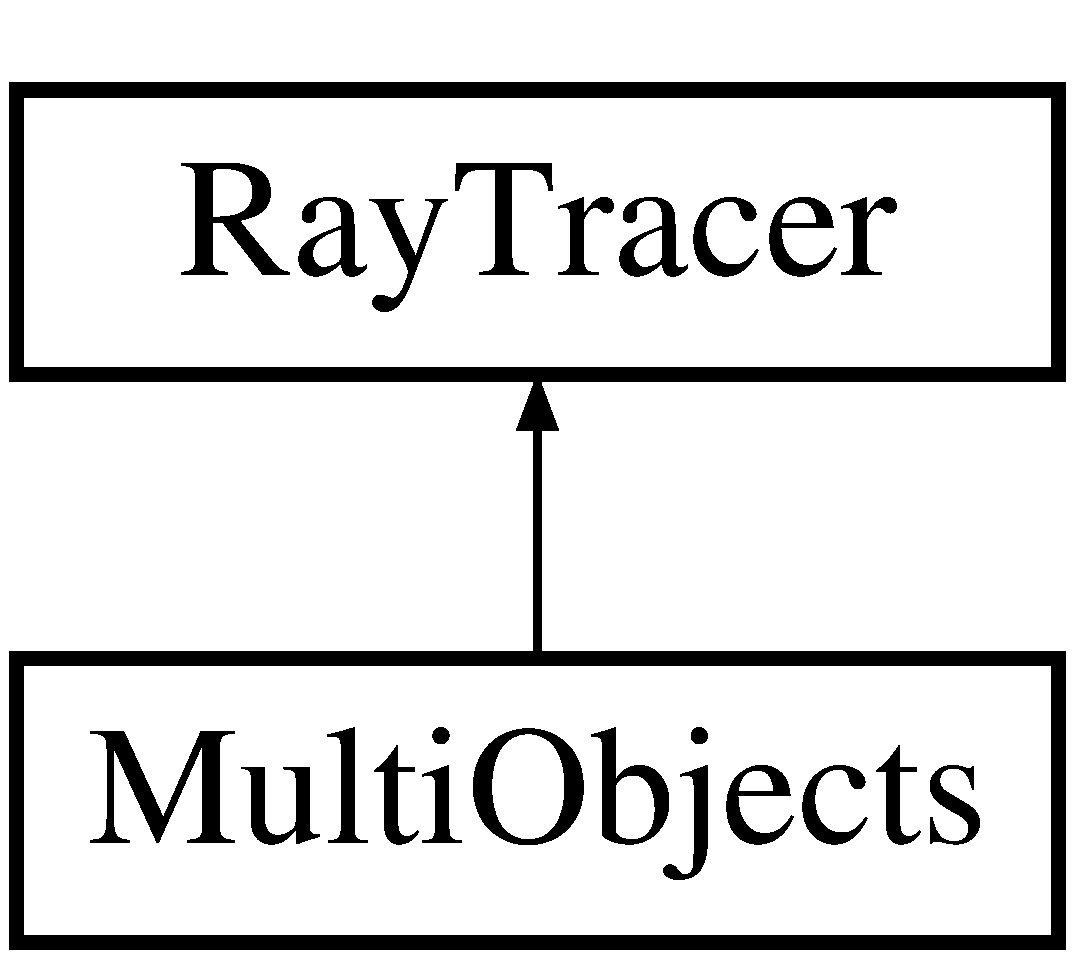
\includegraphics[height=2.000000cm]{class_multi_objects}
\end{center}
\end{figure}
\subsection*{Public Member Functions}
\begin{DoxyCompactItemize}
\item 
\hyperlink{class_multi_objects_a20d6708c1c945bd058ab9bd5840eb8e3}{Multi\-Objects} (\hyperlink{class_world}{World} $\ast$\hyperlink{class_ray_tracer_a0f6b1f71e4ba4aa387c8bffe0b916c1b}{world})
\item 
\hyperlink{class_r_g_b_color}{R\-G\-B\-Color} \hyperlink{class_multi_objects_aaa2b5692917976c50f7a9a33947a40cd}{Trace\-Ray} (const \hyperlink{class_ray}{Ray} \&ray) const 
\end{DoxyCompactItemize}
\subsection*{Additional Inherited Members}


\subsection{Constructor \& Destructor Documentation}
\hypertarget{class_multi_objects_a20d6708c1c945bd058ab9bd5840eb8e3}{\index{Multi\-Objects@{Multi\-Objects}!Multi\-Objects@{Multi\-Objects}}
\index{Multi\-Objects@{Multi\-Objects}!MultiObjects@{Multi\-Objects}}
\subsubsection[{Multi\-Objects}]{\setlength{\rightskip}{0pt plus 5cm}Multi\-Objects\-::\-Multi\-Objects (
\begin{DoxyParamCaption}
\item[{{\bf World} $\ast$}]{world}
\end{DoxyParamCaption}
)}}\label{class_multi_objects_a20d6708c1c945bd058ab9bd5840eb8e3}


\subsection{Member Function Documentation}
\hypertarget{class_multi_objects_aaa2b5692917976c50f7a9a33947a40cd}{\index{Multi\-Objects@{Multi\-Objects}!Trace\-Ray@{Trace\-Ray}}
\index{Trace\-Ray@{Trace\-Ray}!MultiObjects@{Multi\-Objects}}
\subsubsection[{Trace\-Ray}]{\setlength{\rightskip}{0pt plus 5cm}{\bf R\-G\-B\-Color} Multi\-Objects\-::\-Trace\-Ray (
\begin{DoxyParamCaption}
\item[{const {\bf Ray} \&}]{ray}
\end{DoxyParamCaption}
) const\hspace{0.3cm}{\ttfamily [virtual]}}}\label{class_multi_objects_aaa2b5692917976c50f7a9a33947a40cd}


Reimplemented from \hyperlink{class_ray_tracer_a7c884ab374008f3384f18cd6ee328d25}{Ray\-Tracer}.



The documentation for this class was generated from the following files\-:\begin{DoxyCompactItemize}
\item 
raytracer/include/tracer/\hyperlink{_multi_objects_8h}{Multi\-Objects.\-h}\item 
raytracer/source/common/tracer/\hyperlink{_multi_objects_8cpp}{Multi\-Objects.\-cpp}\end{DoxyCompactItemize}

\hypertarget{struct_pixel}{\section{Pixel Struct Reference}
\label{struct_pixel}\index{Pixel@{Pixel}}
}


{\ttfamily \#include $<$Image\-Buffer\-P\-N\-G.\-h$>$}

\subsection*{Public Attributes}
\begin{DoxyCompactItemize}
\item 
uint32\-\_\-t \hyperlink{struct_pixel_a149e152e0e732eec676e90285e7d3502}{color}
\end{DoxyCompactItemize}


\subsection{Member Data Documentation}
\hypertarget{struct_pixel_a149e152e0e732eec676e90285e7d3502}{\index{Pixel@{Pixel}!color@{color}}
\index{color@{color}!Pixel@{Pixel}}
\subsubsection[{color}]{\setlength{\rightskip}{0pt plus 5cm}uint32\-\_\-t Pixel\-::color}}\label{struct_pixel_a149e152e0e732eec676e90285e7d3502}


The documentation for this struct was generated from the following file\-:\begin{DoxyCompactItemize}
\item 
raytracer/include/\hyperlink{_image_buffer_p_n_g_8h}{Image\-Buffer\-P\-N\-G.\-h}\end{DoxyCompactItemize}

\hypertarget{class_plane}{\section{Plane Class Reference}
\label{class_plane}\index{Plane@{Plane}}
}


{\ttfamily \#include $<$Plane.\-h$>$}

Inheritance diagram for Plane\-:\begin{figure}[H]
\begin{center}
\leavevmode
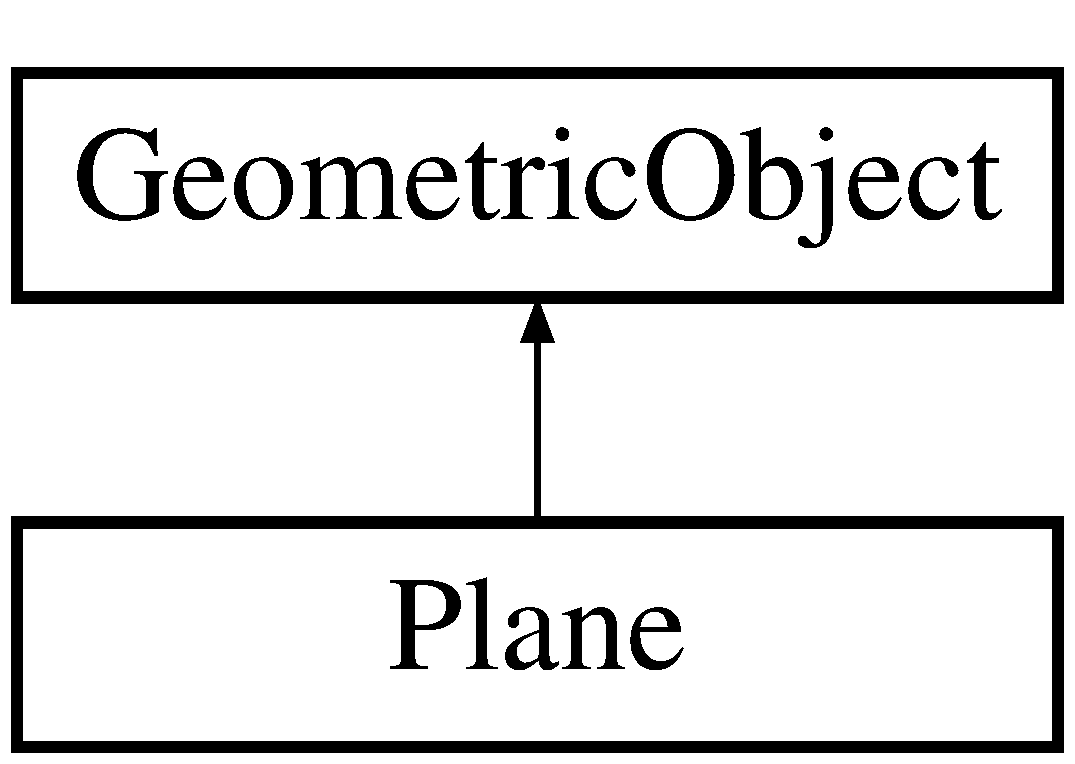
\includegraphics[height=2.000000cm]{class_plane}
\end{center}
\end{figure}
\subsection*{Public Member Functions}
\begin{DoxyCompactItemize}
\item 
bool \hyperlink{class_plane_a51cf933b7cc15b48fa155705d060c541}{Hit} (const \hyperlink{class_ray}{Ray} \&ray, double \&tmin, \hyperlink{class_hit_rec}{Hit\-Rec} \&hr) const 
\end{DoxyCompactItemize}


\subsection{Member Function Documentation}
\hypertarget{class_plane_a51cf933b7cc15b48fa155705d060c541}{\index{Plane@{Plane}!Hit@{Hit}}
\index{Hit@{Hit}!Plane@{Plane}}
\subsubsection[{Hit}]{\setlength{\rightskip}{0pt plus 5cm}bool Plane\-::\-Hit (
\begin{DoxyParamCaption}
\item[{const {\bf Ray} \&}]{ray, }
\item[{double \&}]{tmin, }
\item[{{\bf Hit\-Rec} \&}]{hr}
\end{DoxyParamCaption}
) const\hspace{0.3cm}{\ttfamily [virtual]}}}\label{class_plane_a51cf933b7cc15b48fa155705d060c541}


Implements \hyperlink{class_geometric_object_a6872aae2052bf80cdc0bd87191630b18}{Geometric\-Object}.



The documentation for this class was generated from the following files\-:\begin{DoxyCompactItemize}
\item 
raytracer/include/geom/\hyperlink{_plane_8h}{Plane.\-h}\item 
raytracer/source/common/geom/\hyperlink{_plane_8cpp}{Plane.\-cpp}\end{DoxyCompactItemize}

\hypertarget{class_ray}{\section{Ray Class Reference}
\label{class_ray}\index{Ray@{Ray}}
}


{\ttfamily \#include $<$Ray.\-h$>$}

\subsection*{Public Member Functions}
\begin{DoxyCompactItemize}
\item 
\hyperlink{class_ray_a2e3d2c29f2df4ab3da10da79d4acb852}{Ray} ()
\item 
\hyperlink{class_ray_a8b0e575ce5df046c0c7615c32a96a46f}{$\sim$\-Ray} ()
\end{DoxyCompactItemize}
\subsection*{Public Attributes}
\begin{DoxyCompactItemize}
\item 
glm\-::vec3 \hyperlink{class_ray_afc372b46d562bbe01c1aebc1c3076710}{o}
\item 
glm\-::vec3 \hyperlink{class_ray_a72dcc3f5854ae9cdfeeceb880ea2caea}{d}
\end{DoxyCompactItemize}


\subsection{Constructor \& Destructor Documentation}
\hypertarget{class_ray_a2e3d2c29f2df4ab3da10da79d4acb852}{\index{Ray@{Ray}!Ray@{Ray}}
\index{Ray@{Ray}!Ray@{Ray}}
\subsubsection[{Ray}]{\setlength{\rightskip}{0pt plus 5cm}Ray\-::\-Ray (
\begin{DoxyParamCaption}
{}
\end{DoxyParamCaption}
)}}\label{class_ray_a2e3d2c29f2df4ab3da10da79d4acb852}
\hypertarget{class_ray_a8b0e575ce5df046c0c7615c32a96a46f}{\index{Ray@{Ray}!$\sim$\-Ray@{$\sim$\-Ray}}
\index{$\sim$\-Ray@{$\sim$\-Ray}!Ray@{Ray}}
\subsubsection[{$\sim$\-Ray}]{\setlength{\rightskip}{0pt plus 5cm}Ray\-::$\sim$\-Ray (
\begin{DoxyParamCaption}
{}
\end{DoxyParamCaption}
)}}\label{class_ray_a8b0e575ce5df046c0c7615c32a96a46f}


\subsection{Member Data Documentation}
\hypertarget{class_ray_a72dcc3f5854ae9cdfeeceb880ea2caea}{\index{Ray@{Ray}!d@{d}}
\index{d@{d}!Ray@{Ray}}
\subsubsection[{d}]{\setlength{\rightskip}{0pt plus 5cm}glm\-::vec3 Ray\-::d}}\label{class_ray_a72dcc3f5854ae9cdfeeceb880ea2caea}
\hypertarget{class_ray_afc372b46d562bbe01c1aebc1c3076710}{\index{Ray@{Ray}!o@{o}}
\index{o@{o}!Ray@{Ray}}
\subsubsection[{o}]{\setlength{\rightskip}{0pt plus 5cm}glm\-::vec3 Ray\-::o}}\label{class_ray_afc372b46d562bbe01c1aebc1c3076710}


The documentation for this class was generated from the following files\-:\begin{DoxyCompactItemize}
\item 
raytracer/include/\hyperlink{_ray_8h}{Ray.\-h}\item 
raytracer/source/common/\hyperlink{_ray_8cpp}{Ray.\-cpp}\end{DoxyCompactItemize}

\hypertarget{class_ray_tracer}{\section{Ray\-Tracer Class Reference}
\label{class_ray_tracer}\index{Ray\-Tracer@{Ray\-Tracer}}
}


{\ttfamily \#include $<$Ray\-Tracer.\-h$>$}

Inheritance diagram for Ray\-Tracer\-:\begin{figure}[H]
\begin{center}
\leavevmode
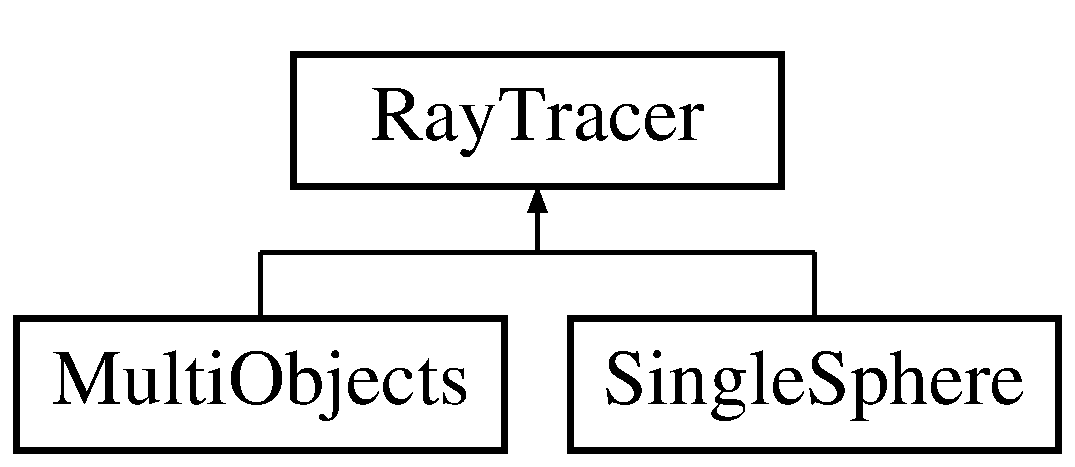
\includegraphics[height=2.000000cm]{class_ray_tracer}
\end{center}
\end{figure}
\subsection*{Public Member Functions}
\begin{DoxyCompactItemize}
\item 
\hyperlink{class_ray_tracer_ad4b0fe2986e8ba61659ab72d8d1e663e}{Ray\-Tracer} (\hyperlink{class_world}{World} $\ast$\hyperlink{class_ray_tracer_a0f6b1f71e4ba4aa387c8bffe0b916c1b}{world})
\item 
\hyperlink{class_ray_tracer_ab5b30fead4f47d46be62bddb4a5283e6}{$\sim$\-Ray\-Tracer} ()
\item 
virtual \hyperlink{class_r_g_b_color}{R\-G\-B\-Color} \hyperlink{class_ray_tracer_a7c884ab374008f3384f18cd6ee328d25}{Trace\-Ray} (const \hyperlink{class_ray}{Ray} \&ray) const 
\end{DoxyCompactItemize}
\subsection*{Protected Attributes}
\begin{DoxyCompactItemize}
\item 
\hyperlink{class_world}{World} $\ast$ \hyperlink{class_ray_tracer_a0f6b1f71e4ba4aa387c8bffe0b916c1b}{world}
\end{DoxyCompactItemize}


\subsection{Constructor \& Destructor Documentation}
\hypertarget{class_ray_tracer_ad4b0fe2986e8ba61659ab72d8d1e663e}{\index{Ray\-Tracer@{Ray\-Tracer}!Ray\-Tracer@{Ray\-Tracer}}
\index{Ray\-Tracer@{Ray\-Tracer}!RayTracer@{Ray\-Tracer}}
\subsubsection[{Ray\-Tracer}]{\setlength{\rightskip}{0pt plus 5cm}Ray\-Tracer\-::\-Ray\-Tracer (
\begin{DoxyParamCaption}
\item[{{\bf World} $\ast$}]{world}
\end{DoxyParamCaption}
)}}\label{class_ray_tracer_ad4b0fe2986e8ba61659ab72d8d1e663e}
\hypertarget{class_ray_tracer_ab5b30fead4f47d46be62bddb4a5283e6}{\index{Ray\-Tracer@{Ray\-Tracer}!$\sim$\-Ray\-Tracer@{$\sim$\-Ray\-Tracer}}
\index{$\sim$\-Ray\-Tracer@{$\sim$\-Ray\-Tracer}!RayTracer@{Ray\-Tracer}}
\subsubsection[{$\sim$\-Ray\-Tracer}]{\setlength{\rightskip}{0pt plus 5cm}Ray\-Tracer\-::$\sim$\-Ray\-Tracer (
\begin{DoxyParamCaption}
{}
\end{DoxyParamCaption}
)}}\label{class_ray_tracer_ab5b30fead4f47d46be62bddb4a5283e6}


\subsection{Member Function Documentation}
\hypertarget{class_ray_tracer_a7c884ab374008f3384f18cd6ee328d25}{\index{Ray\-Tracer@{Ray\-Tracer}!Trace\-Ray@{Trace\-Ray}}
\index{Trace\-Ray@{Trace\-Ray}!RayTracer@{Ray\-Tracer}}
\subsubsection[{Trace\-Ray}]{\setlength{\rightskip}{0pt plus 5cm}{\bf R\-G\-B\-Color} Ray\-Tracer\-::\-Trace\-Ray (
\begin{DoxyParamCaption}
\item[{const {\bf Ray} \&}]{ray}
\end{DoxyParamCaption}
) const\hspace{0.3cm}{\ttfamily [virtual]}}}\label{class_ray_tracer_a7c884ab374008f3384f18cd6ee328d25}


Reimplemented in \hyperlink{class_multi_objects_aaa2b5692917976c50f7a9a33947a40cd}{Multi\-Objects}, and \hyperlink{class_single_sphere_a02d38b2285b90cb7e37325f65337dddb}{Single\-Sphere}.



\subsection{Member Data Documentation}
\hypertarget{class_ray_tracer_a0f6b1f71e4ba4aa387c8bffe0b916c1b}{\index{Ray\-Tracer@{Ray\-Tracer}!world@{world}}
\index{world@{world}!RayTracer@{Ray\-Tracer}}
\subsubsection[{world}]{\setlength{\rightskip}{0pt plus 5cm}{\bf World}$\ast$ Ray\-Tracer\-::world\hspace{0.3cm}{\ttfamily [protected]}}}\label{class_ray_tracer_a0f6b1f71e4ba4aa387c8bffe0b916c1b}


The documentation for this class was generated from the following files\-:\begin{DoxyCompactItemize}
\item 
raytracer/include/tracer/\hyperlink{_ray_tracer_8h}{Ray\-Tracer.\-h}\item 
raytracer/source/common/tracer/\hyperlink{_ray_tracer_8cpp}{Ray\-Tracer.\-cpp}\end{DoxyCompactItemize}

\hypertarget{class_r_g_b_color}{\section{R\-G\-B\-Color Class Reference}
\label{class_r_g_b_color}\index{R\-G\-B\-Color@{R\-G\-B\-Color}}
}


{\ttfamily \#include $<$R\-G\-B\-Color.\-h$>$}

\subsection*{Public Member Functions}
\begin{DoxyCompactItemize}
\item 
\hyperlink{class_r_g_b_color_a9383ce7b63b0a6ada5d4e54e16adf733}{R\-G\-B\-Color} ()
\item 
\hyperlink{class_r_g_b_color_a71d9de2c5f250a724d5b6d9987a601d8}{R\-G\-B\-Color} (const glm\-::vec3 \&color)
\item 
glm\-::vec3 \hyperlink{class_r_g_b_color_a76dfd542cdc5adf37c3c9c44b9e09832}{Get\-R\-G\-B\-Components} () const 
\item 
uint32\-\_\-t \hyperlink{class_r_g_b_color_aec124d79bc012abfc05deb11aedff25f}{Get\-R\-G\-B\-A\-Int\-Packed} () const 
\end{DoxyCompactItemize}
\subsection*{Static Public Attributes}
\begin{DoxyCompactItemize}
\item 
static \hyperlink{class_r_g_b_color}{R\-G\-B\-Color} \hyperlink{class_r_g_b_color_a39194ee333c3c6b2b499f7c320025c34}{black}
\item 
static \hyperlink{class_r_g_b_color}{R\-G\-B\-Color} \hyperlink{class_r_g_b_color_abf657524d06ec0fdb58568a548f12f8b}{red}
\item 
static \hyperlink{class_r_g_b_color}{R\-G\-B\-Color} \hyperlink{class_r_g_b_color_a850de47dd0a7df77ca32a0b5cc6703b7}{yellow}
\end{DoxyCompactItemize}


\subsection{Constructor \& Destructor Documentation}
\hypertarget{class_r_g_b_color_a9383ce7b63b0a6ada5d4e54e16adf733}{\index{R\-G\-B\-Color@{R\-G\-B\-Color}!R\-G\-B\-Color@{R\-G\-B\-Color}}
\index{R\-G\-B\-Color@{R\-G\-B\-Color}!RGBColor@{R\-G\-B\-Color}}
\subsubsection[{R\-G\-B\-Color}]{\setlength{\rightskip}{0pt plus 5cm}R\-G\-B\-Color\-::\-R\-G\-B\-Color (
\begin{DoxyParamCaption}
{}
\end{DoxyParamCaption}
)}}\label{class_r_g_b_color_a9383ce7b63b0a6ada5d4e54e16adf733}
\hypertarget{class_r_g_b_color_a71d9de2c5f250a724d5b6d9987a601d8}{\index{R\-G\-B\-Color@{R\-G\-B\-Color}!R\-G\-B\-Color@{R\-G\-B\-Color}}
\index{R\-G\-B\-Color@{R\-G\-B\-Color}!RGBColor@{R\-G\-B\-Color}}
\subsubsection[{R\-G\-B\-Color}]{\setlength{\rightskip}{0pt plus 5cm}R\-G\-B\-Color\-::\-R\-G\-B\-Color (
\begin{DoxyParamCaption}
\item[{const glm\-::vec3 \&}]{color}
\end{DoxyParamCaption}
)}}\label{class_r_g_b_color_a71d9de2c5f250a724d5b6d9987a601d8}


\subsection{Member Function Documentation}
\hypertarget{class_r_g_b_color_aec124d79bc012abfc05deb11aedff25f}{\index{R\-G\-B\-Color@{R\-G\-B\-Color}!Get\-R\-G\-B\-A\-Int\-Packed@{Get\-R\-G\-B\-A\-Int\-Packed}}
\index{Get\-R\-G\-B\-A\-Int\-Packed@{Get\-R\-G\-B\-A\-Int\-Packed}!RGBColor@{R\-G\-B\-Color}}
\subsubsection[{Get\-R\-G\-B\-A\-Int\-Packed}]{\setlength{\rightskip}{0pt plus 5cm}uint32\-\_\-t R\-G\-B\-Color\-::\-Get\-R\-G\-B\-A\-Int\-Packed (
\begin{DoxyParamCaption}
{}
\end{DoxyParamCaption}
) const}}\label{class_r_g_b_color_aec124d79bc012abfc05deb11aedff25f}
\hypertarget{class_r_g_b_color_a76dfd542cdc5adf37c3c9c44b9e09832}{\index{R\-G\-B\-Color@{R\-G\-B\-Color}!Get\-R\-G\-B\-Components@{Get\-R\-G\-B\-Components}}
\index{Get\-R\-G\-B\-Components@{Get\-R\-G\-B\-Components}!RGBColor@{R\-G\-B\-Color}}
\subsubsection[{Get\-R\-G\-B\-Components}]{\setlength{\rightskip}{0pt plus 5cm}glm\-::vec3 R\-G\-B\-Color\-::\-Get\-R\-G\-B\-Components (
\begin{DoxyParamCaption}
{}
\end{DoxyParamCaption}
) const}}\label{class_r_g_b_color_a76dfd542cdc5adf37c3c9c44b9e09832}


\subsection{Member Data Documentation}
\hypertarget{class_r_g_b_color_a39194ee333c3c6b2b499f7c320025c34}{\index{R\-G\-B\-Color@{R\-G\-B\-Color}!black@{black}}
\index{black@{black}!RGBColor@{R\-G\-B\-Color}}
\subsubsection[{black}]{\setlength{\rightskip}{0pt plus 5cm}{\bf R\-G\-B\-Color} R\-G\-B\-Color\-::black\hspace{0.3cm}{\ttfamily [static]}}}\label{class_r_g_b_color_a39194ee333c3c6b2b499f7c320025c34}
\hypertarget{class_r_g_b_color_abf657524d06ec0fdb58568a548f12f8b}{\index{R\-G\-B\-Color@{R\-G\-B\-Color}!red@{red}}
\index{red@{red}!RGBColor@{R\-G\-B\-Color}}
\subsubsection[{red}]{\setlength{\rightskip}{0pt plus 5cm}{\bf R\-G\-B\-Color} R\-G\-B\-Color\-::red\hspace{0.3cm}{\ttfamily [static]}}}\label{class_r_g_b_color_abf657524d06ec0fdb58568a548f12f8b}
\hypertarget{class_r_g_b_color_a850de47dd0a7df77ca32a0b5cc6703b7}{\index{R\-G\-B\-Color@{R\-G\-B\-Color}!yellow@{yellow}}
\index{yellow@{yellow}!RGBColor@{R\-G\-B\-Color}}
\subsubsection[{yellow}]{\setlength{\rightskip}{0pt plus 5cm}{\bf R\-G\-B\-Color} R\-G\-B\-Color\-::yellow\hspace{0.3cm}{\ttfamily [static]}}}\label{class_r_g_b_color_a850de47dd0a7df77ca32a0b5cc6703b7}


The documentation for this class was generated from the following files\-:\begin{DoxyCompactItemize}
\item 
raytracer/include/\hyperlink{_r_g_b_color_8h}{R\-G\-B\-Color.\-h}\item 
raytracer/source/common/\hyperlink{_r_g_b_color_8cpp}{R\-G\-B\-Color.\-cpp}\end{DoxyCompactItemize}

\hypertarget{class_single_sphere}{\section{Single\-Sphere Class Reference}
\label{class_single_sphere}\index{Single\-Sphere@{Single\-Sphere}}
}


{\ttfamily \#include $<$Single\-Sphere.\-h$>$}

Inheritance diagram for Single\-Sphere\-:\begin{figure}[H]
\begin{center}
\leavevmode
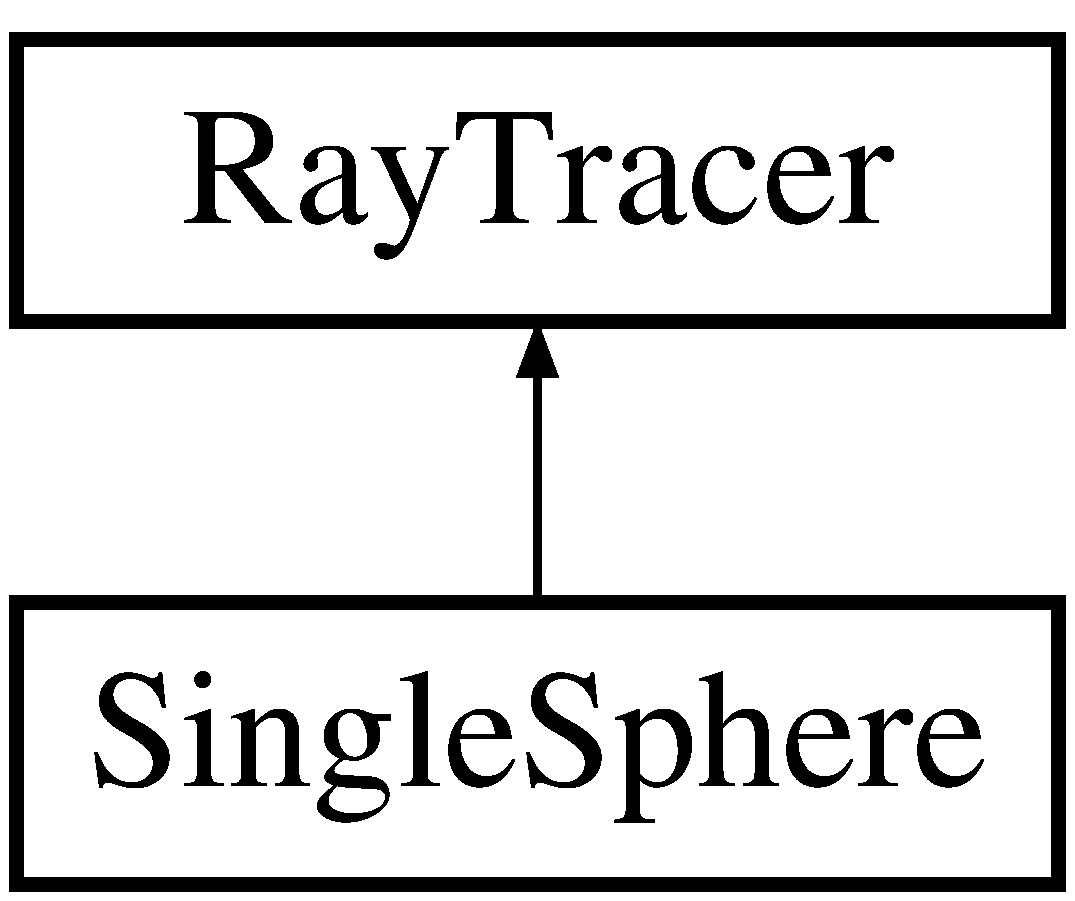
\includegraphics[height=2.000000cm]{class_single_sphere}
\end{center}
\end{figure}
\subsection*{Public Member Functions}
\begin{DoxyCompactItemize}
\item 
\hyperlink{class_single_sphere_a8005ed7d19eeefc86e2952df3d7b0c45}{Single\-Sphere} (\hyperlink{class_world}{World} $\ast$\hyperlink{class_ray_tracer_a0f6b1f71e4ba4aa387c8bffe0b916c1b}{world})
\item 
\hyperlink{class_r_g_b_color}{R\-G\-B\-Color} \hyperlink{class_single_sphere_a02d38b2285b90cb7e37325f65337dddb}{Trace\-Ray} (const \hyperlink{class_ray}{Ray} \&ray) const 
\end{DoxyCompactItemize}
\subsection*{Additional Inherited Members}


\subsection{Constructor \& Destructor Documentation}
\hypertarget{class_single_sphere_a8005ed7d19eeefc86e2952df3d7b0c45}{\index{Single\-Sphere@{Single\-Sphere}!Single\-Sphere@{Single\-Sphere}}
\index{Single\-Sphere@{Single\-Sphere}!SingleSphere@{Single\-Sphere}}
\subsubsection[{Single\-Sphere}]{\setlength{\rightskip}{0pt plus 5cm}Single\-Sphere\-::\-Single\-Sphere (
\begin{DoxyParamCaption}
\item[{{\bf World} $\ast$}]{world}
\end{DoxyParamCaption}
)}}\label{class_single_sphere_a8005ed7d19eeefc86e2952df3d7b0c45}


\subsection{Member Function Documentation}
\hypertarget{class_single_sphere_a02d38b2285b90cb7e37325f65337dddb}{\index{Single\-Sphere@{Single\-Sphere}!Trace\-Ray@{Trace\-Ray}}
\index{Trace\-Ray@{Trace\-Ray}!SingleSphere@{Single\-Sphere}}
\subsubsection[{Trace\-Ray}]{\setlength{\rightskip}{0pt plus 5cm}{\bf R\-G\-B\-Color} Single\-Sphere\-::\-Trace\-Ray (
\begin{DoxyParamCaption}
\item[{const {\bf Ray} \&}]{ray}
\end{DoxyParamCaption}
) const\hspace{0.3cm}{\ttfamily [virtual]}}}\label{class_single_sphere_a02d38b2285b90cb7e37325f65337dddb}


Reimplemented from \hyperlink{class_ray_tracer_a7c884ab374008f3384f18cd6ee328d25}{Ray\-Tracer}.



The documentation for this class was generated from the following files\-:\begin{DoxyCompactItemize}
\item 
raytracer/include/tracer/\hyperlink{_single_sphere_8h}{Single\-Sphere.\-h}\item 
raytracer/source/common/tracer/\hyperlink{_single_sphere_8cpp}{Single\-Sphere.\-cpp}\end{DoxyCompactItemize}

\hypertarget{class_sphere}{\section{Sphere Class Reference}
\label{class_sphere}\index{Sphere@{Sphere}}
}


{\ttfamily \#include $<$Sphere.\-h$>$}

Inheritance diagram for Sphere\-:\begin{figure}[H]
\begin{center}
\leavevmode
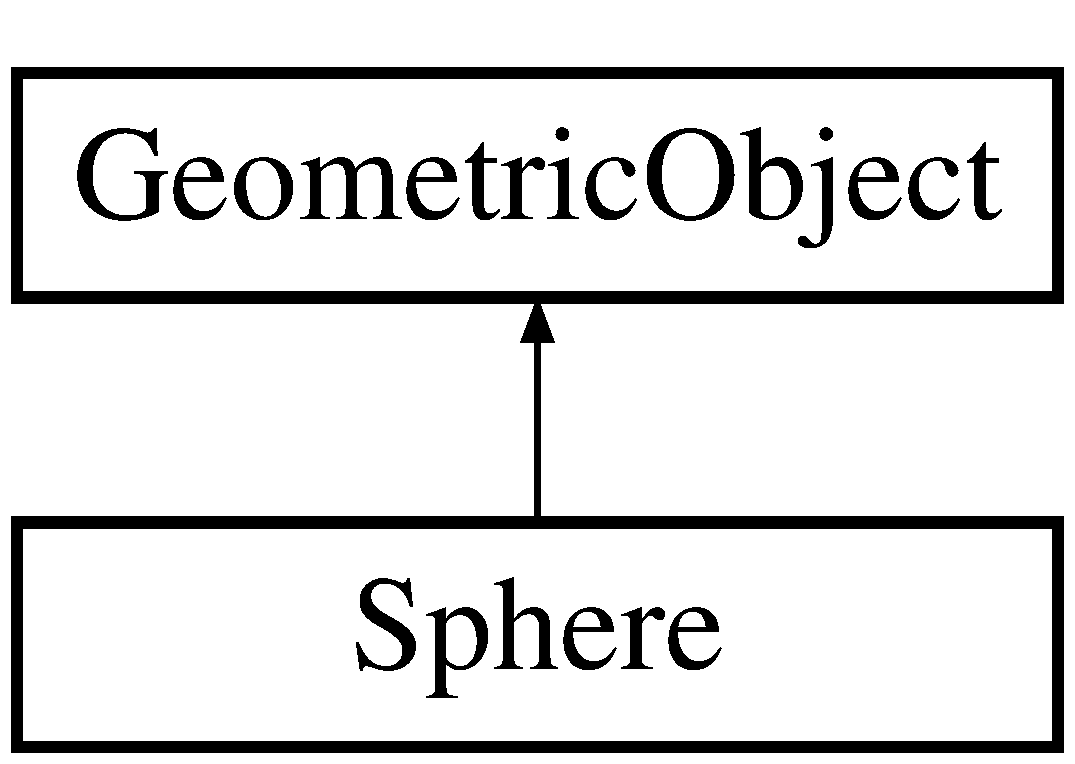
\includegraphics[height=2.000000cm]{class_sphere}
\end{center}
\end{figure}
\subsection*{Public Member Functions}
\begin{DoxyCompactItemize}
\item 
bool \hyperlink{class_sphere_abfe41f348343d7d1dd4a6e5c384c615d}{Hit} (const \hyperlink{class_ray}{Ray} \&ray, double \&tmin, \hyperlink{class_hit_rec}{Hit\-Rec} \&hr) const 
\item 
void \hyperlink{class_sphere_a2b8aef309428ea904c75ce3300a71e09}{Set\-Center} (const glm\-::vec3 \&center)
\item 
void \hyperlink{class_sphere_a3d00bdfc296c57832f92f96c8095f90d}{Set\-Radius} (double radius)
\item 
\hyperlink{class_r_g_b_color}{R\-G\-B\-Color} \hyperlink{class_sphere_a1a1446f19a193f966cb04704faa3c3e8}{Get\-Base\-Color} () override
\end{DoxyCompactItemize}
\subsection*{Public Attributes}
\begin{DoxyCompactItemize}
\item 
\hyperlink{class_r_g_b_color}{R\-G\-B\-Color} \hyperlink{class_sphere_a2dc9c91cfd7554ba873a36c8ca277729}{base\-Color}
\end{DoxyCompactItemize}


\subsection{Member Function Documentation}
\hypertarget{class_sphere_a1a1446f19a193f966cb04704faa3c3e8}{\index{Sphere@{Sphere}!Get\-Base\-Color@{Get\-Base\-Color}}
\index{Get\-Base\-Color@{Get\-Base\-Color}!Sphere@{Sphere}}
\subsubsection[{Get\-Base\-Color}]{\setlength{\rightskip}{0pt plus 5cm}{\bf R\-G\-B\-Color} Sphere\-::\-Get\-Base\-Color (
\begin{DoxyParamCaption}
{}
\end{DoxyParamCaption}
)\hspace{0.3cm}{\ttfamily [override]}, {\ttfamily [virtual]}}}\label{class_sphere_a1a1446f19a193f966cb04704faa3c3e8}


Implements \hyperlink{class_geometric_object_a5971a505ae42f3c916b1f5428b4b3ce1}{Geometric\-Object}.

\hypertarget{class_sphere_abfe41f348343d7d1dd4a6e5c384c615d}{\index{Sphere@{Sphere}!Hit@{Hit}}
\index{Hit@{Hit}!Sphere@{Sphere}}
\subsubsection[{Hit}]{\setlength{\rightskip}{0pt plus 5cm}bool Sphere\-::\-Hit (
\begin{DoxyParamCaption}
\item[{const {\bf Ray} \&}]{ray, }
\item[{double \&}]{tmin, }
\item[{{\bf Hit\-Rec} \&}]{hr}
\end{DoxyParamCaption}
) const\hspace{0.3cm}{\ttfamily [virtual]}}}\label{class_sphere_abfe41f348343d7d1dd4a6e5c384c615d}


Implements \hyperlink{class_geometric_object_a6872aae2052bf80cdc0bd87191630b18}{Geometric\-Object}.

\hypertarget{class_sphere_a2b8aef309428ea904c75ce3300a71e09}{\index{Sphere@{Sphere}!Set\-Center@{Set\-Center}}
\index{Set\-Center@{Set\-Center}!Sphere@{Sphere}}
\subsubsection[{Set\-Center}]{\setlength{\rightskip}{0pt plus 5cm}void Sphere\-::\-Set\-Center (
\begin{DoxyParamCaption}
\item[{const glm\-::vec3 \&}]{center}
\end{DoxyParamCaption}
)}}\label{class_sphere_a2b8aef309428ea904c75ce3300a71e09}
\hypertarget{class_sphere_a3d00bdfc296c57832f92f96c8095f90d}{\index{Sphere@{Sphere}!Set\-Radius@{Set\-Radius}}
\index{Set\-Radius@{Set\-Radius}!Sphere@{Sphere}}
\subsubsection[{Set\-Radius}]{\setlength{\rightskip}{0pt plus 5cm}void Sphere\-::\-Set\-Radius (
\begin{DoxyParamCaption}
\item[{double}]{radius}
\end{DoxyParamCaption}
)}}\label{class_sphere_a3d00bdfc296c57832f92f96c8095f90d}


\subsection{Member Data Documentation}
\hypertarget{class_sphere_a2dc9c91cfd7554ba873a36c8ca277729}{\index{Sphere@{Sphere}!base\-Color@{base\-Color}}
\index{base\-Color@{base\-Color}!Sphere@{Sphere}}
\subsubsection[{base\-Color}]{\setlength{\rightskip}{0pt plus 5cm}{\bf R\-G\-B\-Color} Sphere\-::base\-Color}}\label{class_sphere_a2dc9c91cfd7554ba873a36c8ca277729}


The documentation for this class was generated from the following files\-:\begin{DoxyCompactItemize}
\item 
raytracer/include/geom/\hyperlink{_sphere_8h}{Sphere.\-h}\item 
raytracer/source/common/geom/\hyperlink{_sphere_8cpp}{Sphere.\-cpp}\end{DoxyCompactItemize}

\hypertarget{class_view_plane}{\section{View\-Plane Class Reference}
\label{class_view_plane}\index{View\-Plane@{View\-Plane}}
}


{\ttfamily \#include $<$View\-Plane.\-h$>$}

\subsection*{Public Member Functions}
\begin{DoxyCompactItemize}
\item 
\hyperlink{class_view_plane_ac770dadae1f31408865b409f3128dc57}{View\-Plane} ()
\item 
\hyperlink{class_view_plane}{View\-Plane} \& \hyperlink{class_view_plane_a1170a1aedcc029d61637224e4c2af10c}{Set\-Width} (uint16\-\_\-t width)
\item 
uint16\-\_\-t \hyperlink{class_view_plane_aff20a346c78660cc86dede335b94aa27}{Get\-Width} () const 
\item 
\hyperlink{class_view_plane}{View\-Plane} \& \hyperlink{class_view_plane_addb87fb015c5452f71a164f72bc18229}{Set\-Height} (uint16\-\_\-t height)
\item 
uint16\-\_\-t \hyperlink{class_view_plane_a8bb3fd9d446d4d8e1319d0301b2f60fd}{Get\-Height} () const 
\item 
\hyperlink{class_view_plane}{View\-Plane} \& \hyperlink{class_view_plane_a42ca2f95a1b31497cecb925ef779ac49}{Set\-Pixel\-Size} (float pixsize)
\item 
float \hyperlink{class_view_plane_a806d23e8ce4f7b8ac6e28e4b75c4316e}{Get\-Pixel\-Size} () const 
\end{DoxyCompactItemize}


\subsection{Constructor \& Destructor Documentation}
\hypertarget{class_view_plane_ac770dadae1f31408865b409f3128dc57}{\index{View\-Plane@{View\-Plane}!View\-Plane@{View\-Plane}}
\index{View\-Plane@{View\-Plane}!ViewPlane@{View\-Plane}}
\subsubsection[{View\-Plane}]{\setlength{\rightskip}{0pt plus 5cm}View\-Plane\-::\-View\-Plane (
\begin{DoxyParamCaption}
{}
\end{DoxyParamCaption}
)}}\label{class_view_plane_ac770dadae1f31408865b409f3128dc57}


\subsection{Member Function Documentation}
\hypertarget{class_view_plane_a8bb3fd9d446d4d8e1319d0301b2f60fd}{\index{View\-Plane@{View\-Plane}!Get\-Height@{Get\-Height}}
\index{Get\-Height@{Get\-Height}!ViewPlane@{View\-Plane}}
\subsubsection[{Get\-Height}]{\setlength{\rightskip}{0pt plus 5cm}uint16\-\_\-t View\-Plane\-::\-Get\-Height (
\begin{DoxyParamCaption}
{}
\end{DoxyParamCaption}
) const}}\label{class_view_plane_a8bb3fd9d446d4d8e1319d0301b2f60fd}
\hypertarget{class_view_plane_a806d23e8ce4f7b8ac6e28e4b75c4316e}{\index{View\-Plane@{View\-Plane}!Get\-Pixel\-Size@{Get\-Pixel\-Size}}
\index{Get\-Pixel\-Size@{Get\-Pixel\-Size}!ViewPlane@{View\-Plane}}
\subsubsection[{Get\-Pixel\-Size}]{\setlength{\rightskip}{0pt plus 5cm}float View\-Plane\-::\-Get\-Pixel\-Size (
\begin{DoxyParamCaption}
{}
\end{DoxyParamCaption}
) const}}\label{class_view_plane_a806d23e8ce4f7b8ac6e28e4b75c4316e}
\hypertarget{class_view_plane_aff20a346c78660cc86dede335b94aa27}{\index{View\-Plane@{View\-Plane}!Get\-Width@{Get\-Width}}
\index{Get\-Width@{Get\-Width}!ViewPlane@{View\-Plane}}
\subsubsection[{Get\-Width}]{\setlength{\rightskip}{0pt plus 5cm}uint16\-\_\-t View\-Plane\-::\-Get\-Width (
\begin{DoxyParamCaption}
{}
\end{DoxyParamCaption}
) const}}\label{class_view_plane_aff20a346c78660cc86dede335b94aa27}
\hypertarget{class_view_plane_addb87fb015c5452f71a164f72bc18229}{\index{View\-Plane@{View\-Plane}!Set\-Height@{Set\-Height}}
\index{Set\-Height@{Set\-Height}!ViewPlane@{View\-Plane}}
\subsubsection[{Set\-Height}]{\setlength{\rightskip}{0pt plus 5cm}{\bf View\-Plane} \& View\-Plane\-::\-Set\-Height (
\begin{DoxyParamCaption}
\item[{uint16\-\_\-t}]{height}
\end{DoxyParamCaption}
)}}\label{class_view_plane_addb87fb015c5452f71a164f72bc18229}
\hypertarget{class_view_plane_a42ca2f95a1b31497cecb925ef779ac49}{\index{View\-Plane@{View\-Plane}!Set\-Pixel\-Size@{Set\-Pixel\-Size}}
\index{Set\-Pixel\-Size@{Set\-Pixel\-Size}!ViewPlane@{View\-Plane}}
\subsubsection[{Set\-Pixel\-Size}]{\setlength{\rightskip}{0pt plus 5cm}{\bf View\-Plane} \& View\-Plane\-::\-Set\-Pixel\-Size (
\begin{DoxyParamCaption}
\item[{float}]{pixsize}
\end{DoxyParamCaption}
)}}\label{class_view_plane_a42ca2f95a1b31497cecb925ef779ac49}
\hypertarget{class_view_plane_a1170a1aedcc029d61637224e4c2af10c}{\index{View\-Plane@{View\-Plane}!Set\-Width@{Set\-Width}}
\index{Set\-Width@{Set\-Width}!ViewPlane@{View\-Plane}}
\subsubsection[{Set\-Width}]{\setlength{\rightskip}{0pt plus 5cm}{\bf View\-Plane} \& View\-Plane\-::\-Set\-Width (
\begin{DoxyParamCaption}
\item[{uint16\-\_\-t}]{width}
\end{DoxyParamCaption}
)}}\label{class_view_plane_a1170a1aedcc029d61637224e4c2af10c}


The documentation for this class was generated from the following files\-:\begin{DoxyCompactItemize}
\item 
raytracer/include/\hyperlink{_view_plane_8h}{View\-Plane.\-h}\item 
raytracer/source/common/\hyperlink{_view_plane_8cpp}{View\-Plane.\-cpp}\end{DoxyCompactItemize}

\hypertarget{class_world}{\section{World Class Reference}
\label{class_world}\index{World@{World}}
}


{\ttfamily \#include $<$World.\-h$>$}

\subsection*{Public Member Functions}
\begin{DoxyCompactItemize}
\item 
\hyperlink{class_world_afa39d4e6f714a7a3691ac0c656f5e8a8}{World} ()
\item 
\hyperlink{class_world_a8c73fba541a5817fff65147ba47cd827}{$\sim$\-World} ()
\item 
\hyperlink{class_world}{World} \& \hyperlink{class_world_ab8c2c9c9724071fecb12e07da23ed3a0}{Set\-Output\-Filename} (const char $\ast$outputfile)
\item 
const std\-::string \& \hyperlink{class_world_a83d567953db755169f120b225b86d817}{Get\-Output\-Filename} ()
\item 
void \hyperlink{class_world_a28703ba1eea1c4bb6b796e551b281926}{Build} ()
\item 
void \hyperlink{class_world_af061ea3ec08fd1657945d32eb3e8f6de}{Render\-Scene} ()
\item 
\hyperlink{class_r_g_b_color}{R\-G\-B\-Color} \hyperlink{class_world_a03b7b9c97f4489692dd4bb64deab44ba}{Get\-Background} ()
\item 
void \hyperlink{class_world_a6f05fe0ba61c2757837910243956636e}{Add\-Object} (\hyperlink{class_geometric_object}{Geometric\-Object} $\ast$obj)
\item 
std\-::vector$<$ \hyperlink{class_geometric_object}{Geometric\-Object} $\ast$ $>$ \& \hyperlink{class_world_a9a33c73e51801825b274e217813c5c90}{Get\-Objects} ()
\end{DoxyCompactItemize}
\subsection*{Public Attributes}
\begin{DoxyCompactItemize}
\item 
\hyperlink{class_sphere}{Sphere} \hyperlink{class_world_a9d34d8c2827f2f93f00ea861bdda1c02}{sphere}
\end{DoxyCompactItemize}


\subsection{Constructor \& Destructor Documentation}
\hypertarget{class_world_afa39d4e6f714a7a3691ac0c656f5e8a8}{\index{World@{World}!World@{World}}
\index{World@{World}!World@{World}}
\subsubsection[{World}]{\setlength{\rightskip}{0pt plus 5cm}World\-::\-World (
\begin{DoxyParamCaption}
{}
\end{DoxyParamCaption}
)}}\label{class_world_afa39d4e6f714a7a3691ac0c656f5e8a8}
\hypertarget{class_world_a8c73fba541a5817fff65147ba47cd827}{\index{World@{World}!$\sim$\-World@{$\sim$\-World}}
\index{$\sim$\-World@{$\sim$\-World}!World@{World}}
\subsubsection[{$\sim$\-World}]{\setlength{\rightskip}{0pt plus 5cm}World\-::$\sim$\-World (
\begin{DoxyParamCaption}
{}
\end{DoxyParamCaption}
)}}\label{class_world_a8c73fba541a5817fff65147ba47cd827}


\subsection{Member Function Documentation}
\hypertarget{class_world_a6f05fe0ba61c2757837910243956636e}{\index{World@{World}!Add\-Object@{Add\-Object}}
\index{Add\-Object@{Add\-Object}!World@{World}}
\subsubsection[{Add\-Object}]{\setlength{\rightskip}{0pt plus 5cm}void World\-::\-Add\-Object (
\begin{DoxyParamCaption}
\item[{{\bf Geometric\-Object} $\ast$}]{obj}
\end{DoxyParamCaption}
)}}\label{class_world_a6f05fe0ba61c2757837910243956636e}
\hypertarget{class_world_a28703ba1eea1c4bb6b796e551b281926}{\index{World@{World}!Build@{Build}}
\index{Build@{Build}!World@{World}}
\subsubsection[{Build}]{\setlength{\rightskip}{0pt plus 5cm}void World\-::\-Build (
\begin{DoxyParamCaption}
{}
\end{DoxyParamCaption}
)}}\label{class_world_a28703ba1eea1c4bb6b796e551b281926}
\hypertarget{class_world_a03b7b9c97f4489692dd4bb64deab44ba}{\index{World@{World}!Get\-Background@{Get\-Background}}
\index{Get\-Background@{Get\-Background}!World@{World}}
\subsubsection[{Get\-Background}]{\setlength{\rightskip}{0pt plus 5cm}{\bf R\-G\-B\-Color} World\-::\-Get\-Background (
\begin{DoxyParamCaption}
{}
\end{DoxyParamCaption}
)}}\label{class_world_a03b7b9c97f4489692dd4bb64deab44ba}
\hypertarget{class_world_a9a33c73e51801825b274e217813c5c90}{\index{World@{World}!Get\-Objects@{Get\-Objects}}
\index{Get\-Objects@{Get\-Objects}!World@{World}}
\subsubsection[{Get\-Objects}]{\setlength{\rightskip}{0pt plus 5cm}std\-::vector$<$ {\bf Geometric\-Object} $\ast$ $>$ \& World\-::\-Get\-Objects (
\begin{DoxyParamCaption}
{}
\end{DoxyParamCaption}
)}}\label{class_world_a9a33c73e51801825b274e217813c5c90}
\hypertarget{class_world_a83d567953db755169f120b225b86d817}{\index{World@{World}!Get\-Output\-Filename@{Get\-Output\-Filename}}
\index{Get\-Output\-Filename@{Get\-Output\-Filename}!World@{World}}
\subsubsection[{Get\-Output\-Filename}]{\setlength{\rightskip}{0pt plus 5cm}const std\-::string \& World\-::\-Get\-Output\-Filename (
\begin{DoxyParamCaption}
{}
\end{DoxyParamCaption}
)}}\label{class_world_a83d567953db755169f120b225b86d817}
\hypertarget{class_world_af061ea3ec08fd1657945d32eb3e8f6de}{\index{World@{World}!Render\-Scene@{Render\-Scene}}
\index{Render\-Scene@{Render\-Scene}!World@{World}}
\subsubsection[{Render\-Scene}]{\setlength{\rightskip}{0pt plus 5cm}void World\-::\-Render\-Scene (
\begin{DoxyParamCaption}
{}
\end{DoxyParamCaption}
)}}\label{class_world_af061ea3ec08fd1657945d32eb3e8f6de}
\hypertarget{class_world_ab8c2c9c9724071fecb12e07da23ed3a0}{\index{World@{World}!Set\-Output\-Filename@{Set\-Output\-Filename}}
\index{Set\-Output\-Filename@{Set\-Output\-Filename}!World@{World}}
\subsubsection[{Set\-Output\-Filename}]{\setlength{\rightskip}{0pt plus 5cm}{\bf World} \& World\-::\-Set\-Output\-Filename (
\begin{DoxyParamCaption}
\item[{const char $\ast$}]{outputfile}
\end{DoxyParamCaption}
)}}\label{class_world_ab8c2c9c9724071fecb12e07da23ed3a0}


\subsection{Member Data Documentation}
\hypertarget{class_world_a9d34d8c2827f2f93f00ea861bdda1c02}{\index{World@{World}!sphere@{sphere}}
\index{sphere@{sphere}!World@{World}}
\subsubsection[{sphere}]{\setlength{\rightskip}{0pt plus 5cm}{\bf Sphere} World\-::sphere}}\label{class_world_a9d34d8c2827f2f93f00ea861bdda1c02}


The documentation for this class was generated from the following files\-:\begin{DoxyCompactItemize}
\item 
raytracer/include/\hyperlink{_world_8h}{World.\-h}\item 
raytracer/source/common/\hyperlink{_world_8cpp}{World.\-cpp}\end{DoxyCompactItemize}

\chapter{File Documentation}
\hypertarget{_geometric_object_8h}{\section{raytracer/include/geom/\-Geometric\-Object.h File Reference}
\label{_geometric_object_8h}\index{raytracer/include/geom/\-Geometric\-Object.\-h@{raytracer/include/geom/\-Geometric\-Object.\-h}}
}
\subsection*{Classes}
\begin{DoxyCompactItemize}
\item 
class \hyperlink{class_geometric_object}{Geometric\-Object}
\end{DoxyCompactItemize}

\hypertarget{_plane_8h}{\section{raytracer/include/geom/\-Plane.h File Reference}
\label{_plane_8h}\index{raytracer/include/geom/\-Plane.\-h@{raytracer/include/geom/\-Plane.\-h}}
}
{\ttfamily \#include $<$geom/\-Geometric\-Object.\-h$>$}\\*
\subsection*{Classes}
\begin{DoxyCompactItemize}
\item 
class \hyperlink{class_plane}{Plane}
\end{DoxyCompactItemize}

\hypertarget{_sphere_8h}{\section{raytracer/include/geom/\-Sphere.h File Reference}
\label{_sphere_8h}\index{raytracer/include/geom/\-Sphere.\-h@{raytracer/include/geom/\-Sphere.\-h}}
}
{\ttfamily \#include $<$geom/\-Geometric\-Object.\-h$>$}\\*
{\ttfamily \#include $<$glm/glm.\-hpp$>$}\\*
{\ttfamily \#include $<$R\-G\-B\-Color.\-h$>$}\\*
\subsection*{Classes}
\begin{DoxyCompactItemize}
\item 
class \hyperlink{class_sphere}{Sphere}
\end{DoxyCompactItemize}

\hypertarget{_hit_rec_8h}{\section{raytracer/include/\-Hit\-Rec.h File Reference}
\label{_hit_rec_8h}\index{raytracer/include/\-Hit\-Rec.\-h@{raytracer/include/\-Hit\-Rec.\-h}}
}
{\ttfamily \#include $<$glm/glm.\-hpp$>$}\\*
\subsection*{Classes}
\begin{DoxyCompactItemize}
\item 
class \hyperlink{class_hit_rec}{Hit\-Rec}
\end{DoxyCompactItemize}

\hypertarget{_image_buffer_p_n_g_8h}{\section{raytracer/include/\-Image\-Buffer\-P\-N\-G.h File Reference}
\label{_image_buffer_p_n_g_8h}\index{raytracer/include/\-Image\-Buffer\-P\-N\-G.\-h@{raytracer/include/\-Image\-Buffer\-P\-N\-G.\-h}}
}
{\ttfamily \#include $<$stdint.\-h$>$}\\*
{\ttfamily \#include $<$memory$>$}\\*
\subsection*{Classes}
\begin{DoxyCompactItemize}
\item 
struct \hyperlink{struct_pixel}{Pixel}
\item 
class \hyperlink{class_image_buffer_p_n_g}{Image\-Buffer\-P\-N\-G}
\end{DoxyCompactItemize}

\hypertarget{_ray_8h}{\section{raytracer/include/\-Ray.h File Reference}
\label{_ray_8h}\index{raytracer/include/\-Ray.\-h@{raytracer/include/\-Ray.\-h}}
}
{\ttfamily \#include $<$glm/glm.\-hpp$>$}\\*
\subsection*{Classes}
\begin{DoxyCompactItemize}
\item 
class \hyperlink{class_ray}{Ray}
\end{DoxyCompactItemize}

\hypertarget{_r_g_b_color_8h}{\section{raytracer/include/\-R\-G\-B\-Color.h File Reference}
\label{_r_g_b_color_8h}\index{raytracer/include/\-R\-G\-B\-Color.\-h@{raytracer/include/\-R\-G\-B\-Color.\-h}}
}
{\ttfamily \#include $<$glm/glm.\-hpp$>$}\\*
\subsection*{Classes}
\begin{DoxyCompactItemize}
\item 
class \hyperlink{class_r_g_b_color}{R\-G\-B\-Color}
\end{DoxyCompactItemize}

\hypertarget{_multi_objects_8h}{\section{raytracer/include/tracer/\-Multi\-Objects.h File Reference}
\label{_multi_objects_8h}\index{raytracer/include/tracer/\-Multi\-Objects.\-h@{raytracer/include/tracer/\-Multi\-Objects.\-h}}
}
{\ttfamily \#include $<$tracer/\-Ray\-Tracer.\-h$>$}\\*
\subsection*{Classes}
\begin{DoxyCompactItemize}
\item 
class \hyperlink{class_multi_objects}{Multi\-Objects}
\end{DoxyCompactItemize}

\hypertarget{_ray_tracer_8h}{\section{raytracer/include/tracer/\-Ray\-Tracer.h File Reference}
\label{_ray_tracer_8h}\index{raytracer/include/tracer/\-Ray\-Tracer.\-h@{raytracer/include/tracer/\-Ray\-Tracer.\-h}}
}
{\ttfamily \#include $<$string$>$}\\*
{\ttfamily \#include $<$memory$>$}\\*
\subsection*{Classes}
\begin{DoxyCompactItemize}
\item 
class \hyperlink{class_ray_tracer}{Ray\-Tracer}
\end{DoxyCompactItemize}

\hypertarget{_single_sphere_8h}{\section{raytracer/include/tracer/\-Single\-Sphere.h File Reference}
\label{_single_sphere_8h}\index{raytracer/include/tracer/\-Single\-Sphere.\-h@{raytracer/include/tracer/\-Single\-Sphere.\-h}}
}
{\ttfamily \#include $<$tracer/\-Ray\-Tracer.\-h$>$}\\*
\subsection*{Classes}
\begin{DoxyCompactItemize}
\item 
class \hyperlink{class_single_sphere}{Single\-Sphere}
\end{DoxyCompactItemize}

\hypertarget{_view_plane_8h}{\section{raytracer/include/\-View\-Plane.h File Reference}
\label{_view_plane_8h}\index{raytracer/include/\-View\-Plane.\-h@{raytracer/include/\-View\-Plane.\-h}}
}
{\ttfamily \#include $<$stdint.\-h$>$}\\*
\subsection*{Classes}
\begin{DoxyCompactItemize}
\item 
class \hyperlink{class_view_plane}{View\-Plane}
\end{DoxyCompactItemize}

\hypertarget{_world_8h}{\section{raytracer/include/\-World.h File Reference}
\label{_world_8h}\index{raytracer/include/\-World.\-h@{raytracer/include/\-World.\-h}}
}
{\ttfamily \#include $<$string$>$}\\*
{\ttfamily \#include $<$R\-G\-B\-Color.\-h$>$}\\*
{\ttfamily \#include $<$geom/\-Sphere.\-h$>$}\\*
{\ttfamily \#include $<$vector$>$}\\*
\subsection*{Classes}
\begin{DoxyCompactItemize}
\item 
class \hyperlink{class_world}{World}
\end{DoxyCompactItemize}

\hypertarget{_geometric_object_8cpp}{\section{raytracer/source/common/geom/\-Geometric\-Object.cpp File Reference}
\label{_geometric_object_8cpp}\index{raytracer/source/common/geom/\-Geometric\-Object.\-cpp@{raytracer/source/common/geom/\-Geometric\-Object.\-cpp}}
}
{\ttfamily \#include $<$geom/\-Geometric\-Object.\-h$>$}\\*
{\ttfamily \#include $<$Hit\-Rec.\-h$>$}\\*

\hypertarget{_plane_8cpp}{\section{raytracer/source/common/geom/\-Plane.cpp File Reference}
\label{_plane_8cpp}\index{raytracer/source/common/geom/\-Plane.\-cpp@{raytracer/source/common/geom/\-Plane.\-cpp}}
}
{\ttfamily \#include $<$geom/\-Plane.\-h$>$}\\*

\hypertarget{_sphere_8cpp}{\section{raytracer/source/common/geom/\-Sphere.cpp File Reference}
\label{_sphere_8cpp}\index{raytracer/source/common/geom/\-Sphere.\-cpp@{raytracer/source/common/geom/\-Sphere.\-cpp}}
}
{\ttfamily \#include $<$geom/\-Sphere.\-h$>$}\\*
{\ttfamily \#include $<$Ray.\-h$>$}\\*
{\ttfamily \#include $<$Hit\-Rec.\-h$>$}\\*
{\ttfamily \#include $<$R\-G\-B\-Color.\-h$>$}\\*

\hypertarget{_hit_rec_8cpp}{\section{raytracer/source/common/\-Hit\-Rec.cpp File Reference}
\label{_hit_rec_8cpp}\index{raytracer/source/common/\-Hit\-Rec.\-cpp@{raytracer/source/common/\-Hit\-Rec.\-cpp}}
}
{\ttfamily \#include $<$Hit\-Rec.\-h$>$}\\*

\hypertarget{_image_buffer_p_n_g_8cpp}{\section{raytracer/source/common/\-Image\-Buffer\-P\-N\-G.cpp File Reference}
\label{_image_buffer_p_n_g_8cpp}\index{raytracer/source/common/\-Image\-Buffer\-P\-N\-G.\-cpp@{raytracer/source/common/\-Image\-Buffer\-P\-N\-G.\-cpp}}
}
{\ttfamily \#include $<$Image\-Buffer\-P\-N\-G.\-h$>$}\\*
{\ttfamily \#include $<$memory$>$}\\*
{\ttfamily \#include $<$lodepng.\-h$>$}\\*

\hypertarget{_main_8cpp}{\section{raytracer/source/common/\-Main.cpp File Reference}
\label{_main_8cpp}\index{raytracer/source/common/\-Main.\-cpp@{raytracer/source/common/\-Main.\-cpp}}
}
{\ttfamily \#include $<$cstdio$>$}\\*
{\ttfamily \#include $<$tracer/\-Ray\-Tracer.\-h$>$}\\*
{\ttfamily \#include $<$World.\-h$>$}\\*
\subsection*{Functions}
\begin{DoxyCompactItemize}
\item 
int \hyperlink{_main_8cpp_a3c04138a5bfe5d72780bb7e82a18e627}{main} (int argc, char $\ast$$\ast$argv)
\end{DoxyCompactItemize}


\subsection{Function Documentation}
\hypertarget{_main_8cpp_a3c04138a5bfe5d72780bb7e82a18e627}{\index{Main.\-cpp@{Main.\-cpp}!main@{main}}
\index{main@{main}!Main.cpp@{Main.\-cpp}}
\subsubsection[{main}]{\setlength{\rightskip}{0pt plus 5cm}int main (
\begin{DoxyParamCaption}
\item[{int}]{argc, }
\item[{char $\ast$$\ast$}]{argv}
\end{DoxyParamCaption}
)}}\label{_main_8cpp_a3c04138a5bfe5d72780bb7e82a18e627}

\hypertarget{_ray_8cpp}{\section{raytracer/source/common/\-Ray.cpp File Reference}
\label{_ray_8cpp}\index{raytracer/source/common/\-Ray.\-cpp@{raytracer/source/common/\-Ray.\-cpp}}
}
{\ttfamily \#include $<$Ray.\-h$>$}\\*

\hypertarget{_r_g_b_color_8cpp}{\section{raytracer/source/common/\-R\-G\-B\-Color.cpp File Reference}
\label{_r_g_b_color_8cpp}\index{raytracer/source/common/\-R\-G\-B\-Color.\-cpp@{raytracer/source/common/\-R\-G\-B\-Color.\-cpp}}
}
{\ttfamily \#include $<$R\-G\-B\-Color.\-h$>$}\\*

\hypertarget{_multi_objects_8cpp}{\section{raytracer/source/common/tracer/\-Multi\-Objects.cpp File Reference}
\label{_multi_objects_8cpp}\index{raytracer/source/common/tracer/\-Multi\-Objects.\-cpp@{raytracer/source/common/tracer/\-Multi\-Objects.\-cpp}}
}
{\ttfamily \#include $<$tracer/\-Multi\-Objects.\-h$>$}\\*
{\ttfamily \#include $<$R\-G\-B\-Color.\-h$>$}\\*
{\ttfamily \#include $<$Hit\-Rec.\-h$>$}\\*
{\ttfamily \#include $<$World.\-h$>$}\\*
{\ttfamily \#include $<$cfloat$>$}\\*

\hypertarget{_ray_tracer_8cpp}{\section{raytracer/source/common/tracer/\-Ray\-Tracer.cpp File Reference}
\label{_ray_tracer_8cpp}\index{raytracer/source/common/tracer/\-Ray\-Tracer.\-cpp@{raytracer/source/common/tracer/\-Ray\-Tracer.\-cpp}}
}
{\ttfamily \#include $<$tracer/\-Ray\-Tracer.\-h$>$}\\*
{\ttfamily \#include $<$Image\-Buffer\-P\-N\-G.\-h$>$}\\*
{\ttfamily \#include $<$Ray.\-h$>$}\\*
{\ttfamily \#include $<$World.\-h$>$}\\*
{\ttfamily \#include $<$R\-G\-B\-Color.\-h$>$}\\*

\hypertarget{_single_sphere_8cpp}{\section{raytracer/source/common/tracer/\-Single\-Sphere.cpp File Reference}
\label{_single_sphere_8cpp}\index{raytracer/source/common/tracer/\-Single\-Sphere.\-cpp@{raytracer/source/common/tracer/\-Single\-Sphere.\-cpp}}
}
{\ttfamily \#include $<$tracer/\-Single\-Sphere.\-h$>$}\\*
{\ttfamily \#include $<$R\-G\-B\-Color.\-h$>$}\\*
{\ttfamily \#include $<$Hit\-Rec.\-h$>$}\\*
{\ttfamily \#include $<$World.\-h$>$}\\*

\hypertarget{_view_plane_8cpp}{\section{raytracer/source/common/\-View\-Plane.cpp File Reference}
\label{_view_plane_8cpp}\index{raytracer/source/common/\-View\-Plane.\-cpp@{raytracer/source/common/\-View\-Plane.\-cpp}}
}
{\ttfamily \#include $<$View\-Plane.\-h$>$}\\*

\hypertarget{_world_8cpp}{\section{raytracer/source/common/\-World.cpp File Reference}
\label{_world_8cpp}\index{raytracer/source/common/\-World.\-cpp@{raytracer/source/common/\-World.\-cpp}}
}
{\ttfamily \#include $<$World.\-h$>$}\\*
{\ttfamily \#include $<$Image\-Buffer\-P\-N\-G.\-h$>$}\\*
{\ttfamily \#include $<$View\-Plane.\-h$>$}\\*
{\ttfamily \#include $<$tracer/\-Multi\-Objects.\-h$>$}\\*
{\ttfamily \#include $<$Ray.\-h$>$}\\*

%--- End generated contents ---

% Index
\newpage
\phantomsection
\addcontentsline{toc}{part}{Index}
\printindex

\end{document}
